\subsection{SyntaxSQLNet}

The main goal of developing the SyntaxSQLNet model\cite{DBLP:journals/corr/abs-1810-05237} was to generate complex SQL queries with multiple clauses and generalize them to new databases.
This was achieved through the use of a syntax tree network, which is capable of addressing complex and cross-domain queries.
As is evident in the chart below, the SyntaxSQLNet model is composed of several components, each with its unique function and purpose in generating complex SQL queries. The encoders are table-aware, while the decoders have a history of the SQL generation path.

With a massive 7.3\% improvement in accuracy, SyntaxSQLNet outperformed previous models, such as SQLNet, on the SPIDER dataset.
A cross-domain data augmentation technique was employed to improve accuracy further to generate more variance during training, allowing for a greater degree of accuracy and robustness.

\begin{figure}[htb]
    \centering
    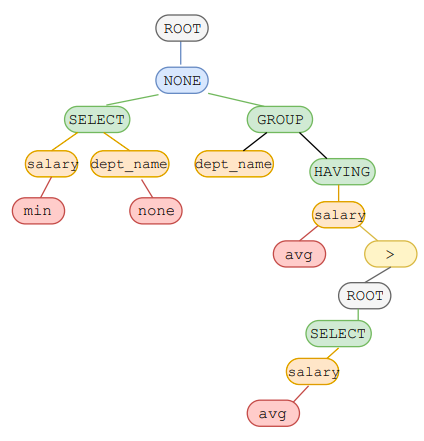
\includegraphics[width=0.5\textwidth]{pics/SyntaxSQLNet/Tree-based.png}
    \caption{Tree-based SQL generator in SyntaxSQLNet\cite{DBLP:journals/corr/abs-1810-05237}}
    \label{fig:tree-based}
\end{figure}

% \begin{figure}[htb]
%     \centering
%     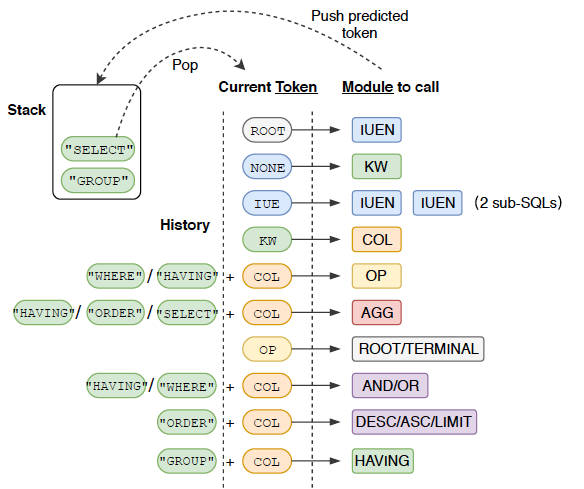
\includegraphics[width=0.8\textwidth]{pics/SyntaxSQLNet/Grammar.png}
%     \caption{Modules defined in SyntaxSQLNet model\cite{DBLP:journals/corr/abs-1810-05237}}
%     \label{fig:grammar}
% \end{figure}

\subsubsection*{SQL Grammar and Attention Mechanism}

To enable the decoder to handle complex queries, SQL grammar is employed in order to allow the decoder to make decisions at each step of recursive decoding. This allows the decoder to determine which module to invoke for the prediction of the following SQL token, taking into account the history of SQL path generation, the current SQL tokens, and the attention mechanism. The attention mechanism is used to encode the question representation, which is then applied to the SQL path history encoding. This is advantageous as it allows for a more detailed representation of the query to be created, which in turn leads to more efficient and accurate responses.

% \subsubsection*{Data Augmentation}

% Despite SPIDER's large dataset, it lacks complex queries. To achieve proper generalization, cross-domain datasets are used for data augmentation. The SPIDER dataset is used to prepare a list of patterns for natural language questions and corresponding SQL queries. The SPIDER model, using syntaxSQLNet decoding history, reaches 27.2\% accuracy, an increase of 12.4\% compared to previous models such as SQLNet.